% ============================================================
%  Hands-On 1 — Pengenalan Antarmuka Sistem Operasi dan Virtual Machine
% ============================================================

\chapter{Instalasi Ubuntu pada VirtualBox}
\label{chap:handson-01}

% --- 1. Tugas ---
\section{Tugas}

Jawablah pertanyaan-pertanyaan berikut berdasarkan hasil praktikum Anda.
Sertakan bukti berupa \textit{screenshot} atau penggalan keluaran terminal
yang relevan pada setiap jawaban.

\begin{enumerate}
    \item \textbf{Tujuan dan Output Praktikum}\\[0.3cm]
    \textbf{A. Tujuan Praktikum}
    \begin{enumerate}[nosep]
        \item Menjelaskan konsep sistem operasi sebagai pengelola sumber daya komputer.
        \item Mengidentifikasi fungsi utama sistem operasi (manajemen proses, memori, berkas, dan I/O).
        \item Membedakan antarmuka GUI dan CLI berdasarkan karakteristik serta penggunaannya.
        \item Memahami konsep dasar Virtual Machine dan peranannya dalam praktikum sistem operasi.
    \end{enumerate}
    \textbf{B. Output Praktikum}
    \begin{enumerate}[nosep]
        \item Ringkasan Pemahaman Sistem Operasi
        \item Perbedaan GUI dan CLI
    \end{enumerate}

    \item \textbf{Alat dan Bahan}
    \begin{enumerate}[nosep]
        \item \textbf{Perangkat Keras:}
        \begin{enumerate}[nosep]
            \item Laptop atau PC dengan prosesor minimal dual-core.
            \item RAM minimal 4 GB (disarankan 8 GB untuk kinerja optimal).
            \item Ruang penyimpanan kosong minimal 25 GB.
        \end{enumerate}
        \item \textbf{Perangkat Lunak:}
        \begin{enumerate}[nosep]
            \item Sistem Operasi utama (Windows, macOS, atau Linux) sebagai Host OS.
            \item Oracle VM VirtualBox.
            \item File ISO Ubuntu.
        \end{enumerate}
    \end{enumerate}

    \item \textbf{Langkah-langkah Praktikum}\\[0.3cm]
    \textbf{A. Instalasi VirtualBox}
    \begin{enumerate}[nosep]
        \item Buka web resmi Ubuntu di https://ubuntu.com/download/desktop dan download file ISO Ubuntu Desktop.\\
        \begin{figure}[H]
            \centering
            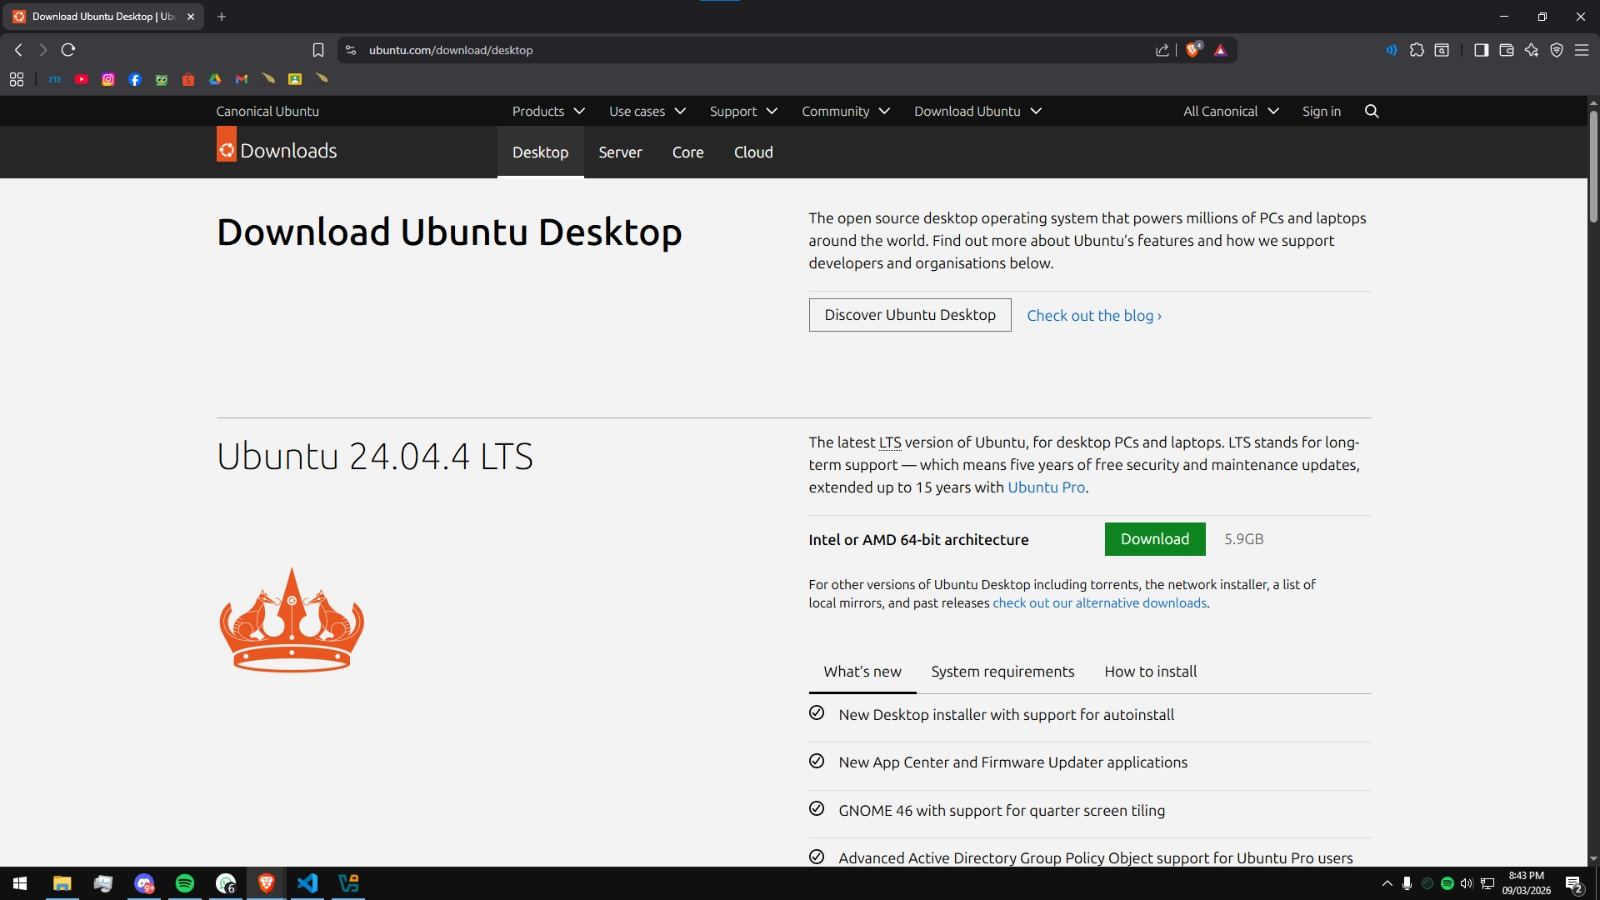
\includegraphics[width=0.85\textwidth]{Figure/UbuntuDownload.jpeg}
            \caption{Web resmi Ubuntu}
        \end{figure}
        \item Download VirtualBox dari web resmi https://www.virtualbox.org dan ikuti petunjuk instalasi sesuai dengan sistem operasi yang digunakan.\\
        \begin{figure}[H]
            \centering
            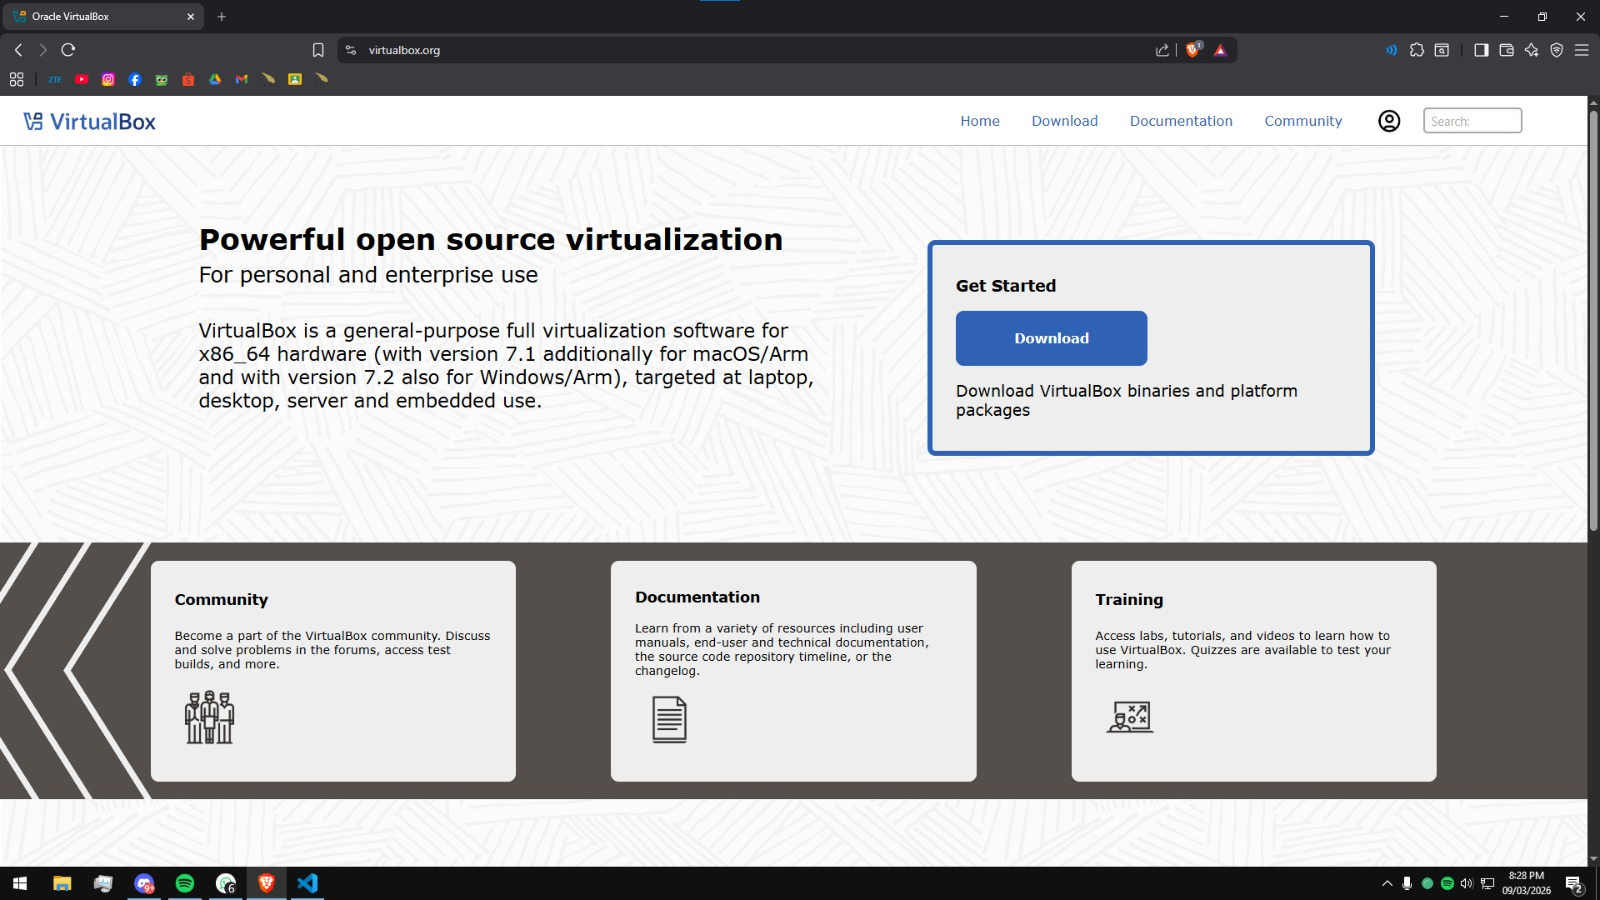
\includegraphics[width=0.85\textwidth]{Figure/VMDownload.jpeg}
            \caption{Web resmi VirtualBox}
        \end{figure}
        \item Setelah instalasi selesai, buka VirtualBox dan buat mesin virtual baru. Berikan nama, dan pilih ISO Image Ubuntu yang telah didownload sebelumnya.\\
        \begin{figure}[H]
            \centering
            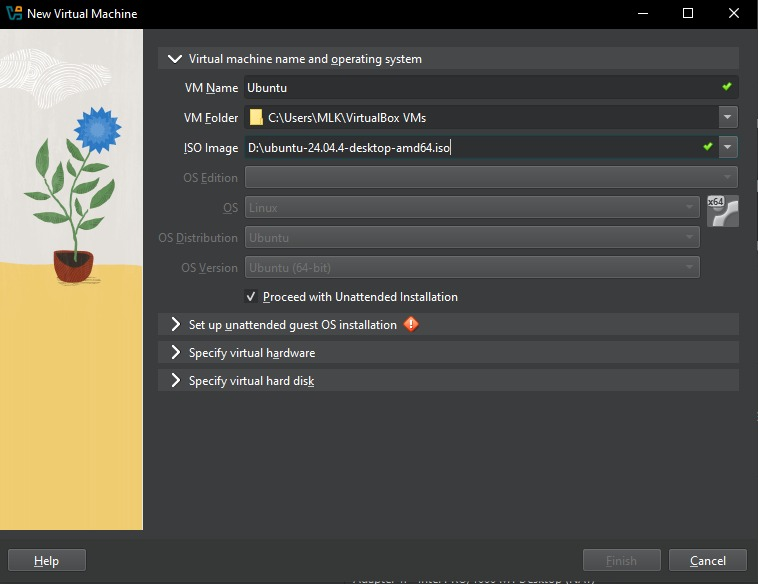
\includegraphics[width=0.85\textwidth]{Figure/1.png}
            \caption{Pembuatan VM baru}
        \end{figure}
        \item Pada bagian kedua, buat username dan password untuk akun Ubuntu yang akan dibuat.\\
        \begin{figure}[H]
            \centering
            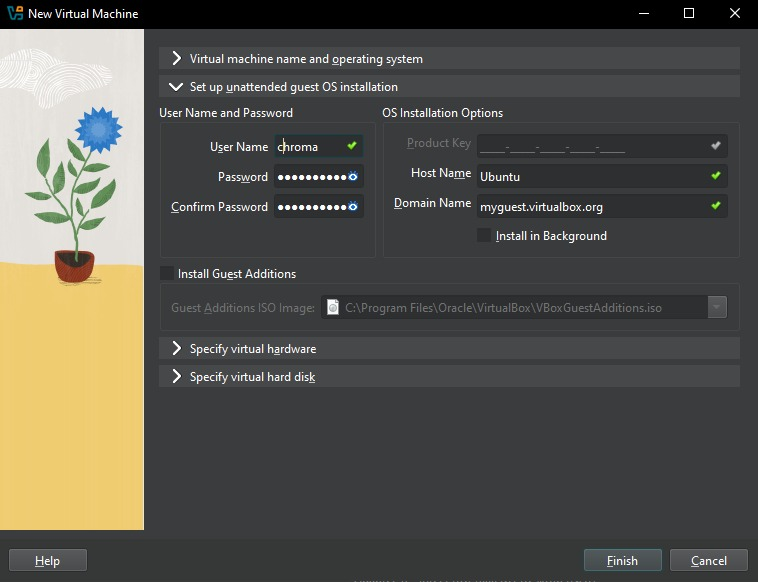
\includegraphics[width=0.85\textwidth]{Figure/2.png}
            \caption{Pembuatan akun Ubuntu}
        \end{figure}
        \item Pada bagian ketiga, alokasikan RAM minimal 2048 MB dan CPU minimal 2 core.\\
        \begin{figure}[H]
            \centering
            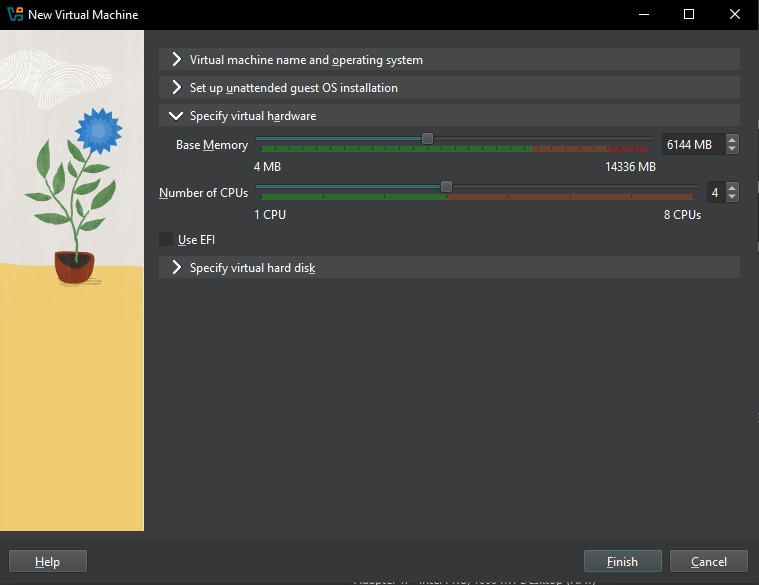
\includegraphics[width=0.85\textwidth]{Figure/3.png}
            \caption{Alokasi RAM dan CPU}
        \end{figure}
        \item Pada bagian terakhir, alokasikan penyimpanan sesuai kebutuhan, misal 25Gb.
        \begin{figure}[H]
            \centering
            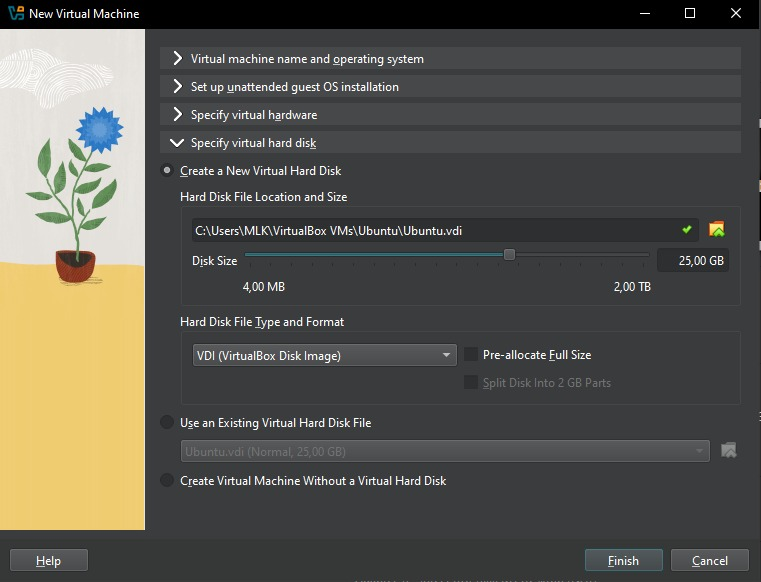
\includegraphics[width=0.85\textwidth]{Figure/4.png}
            \caption{Alokasi penyimpanan}
        \end{figure}
        \item Setelah semua pengaturan selesai, klik "Create" untuk membuat VM.
    \end{enumerate}

    \item \textbf{Eksplorasi Mandiri}
    \begin{enumerate}[nosep]
        \item Mengikuti proses instalasi Ubuntu hingga selesai.\\
        \begin{figure}[H]
            \centering
            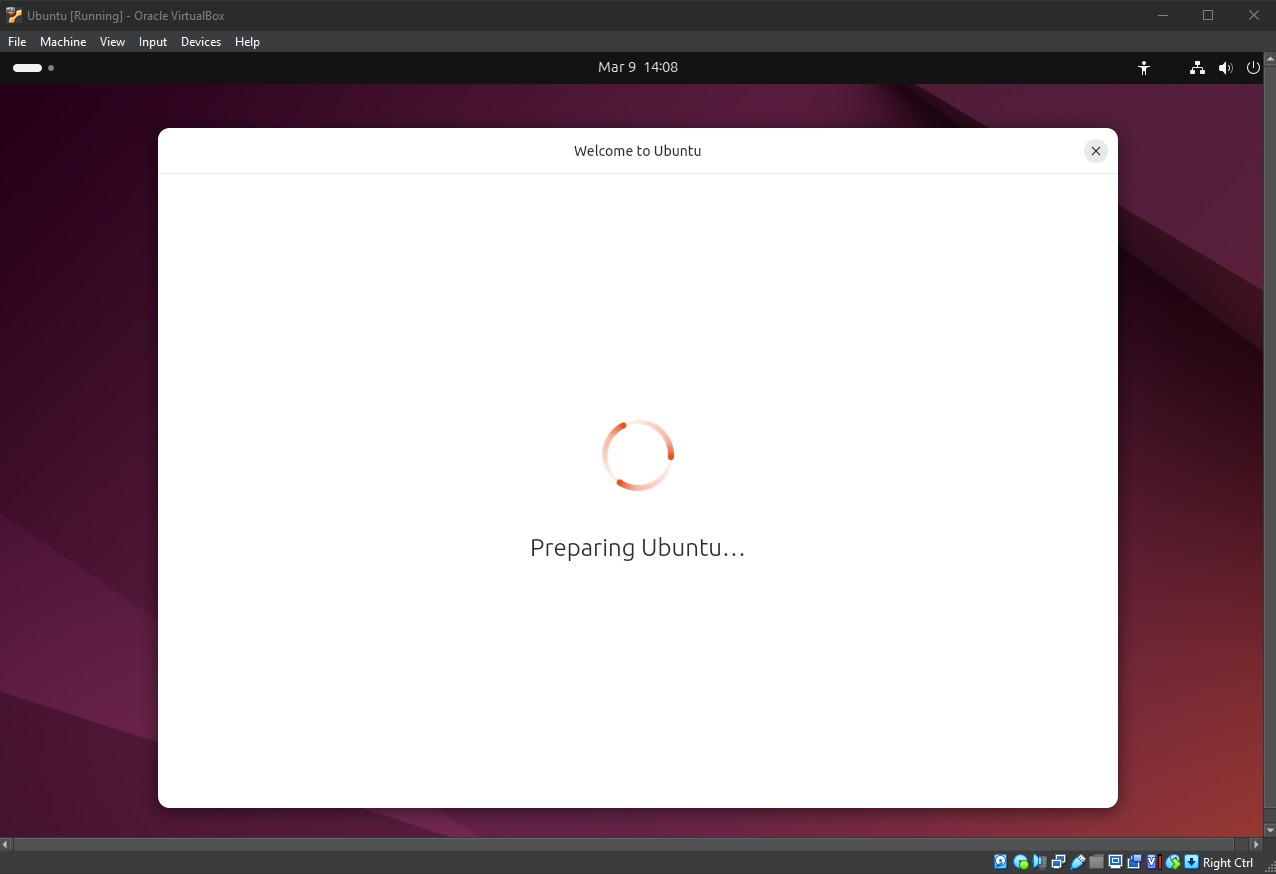
\includegraphics[width=0.85\textwidth]{Figure/Ubuntu1.png}
            \caption{Proses instalasi Ubuntu}
        \end{figure}
        \item Eksplorasi software Ubuntu (misal Firefox).\\
        \begin{figure}[H]
            \centering
            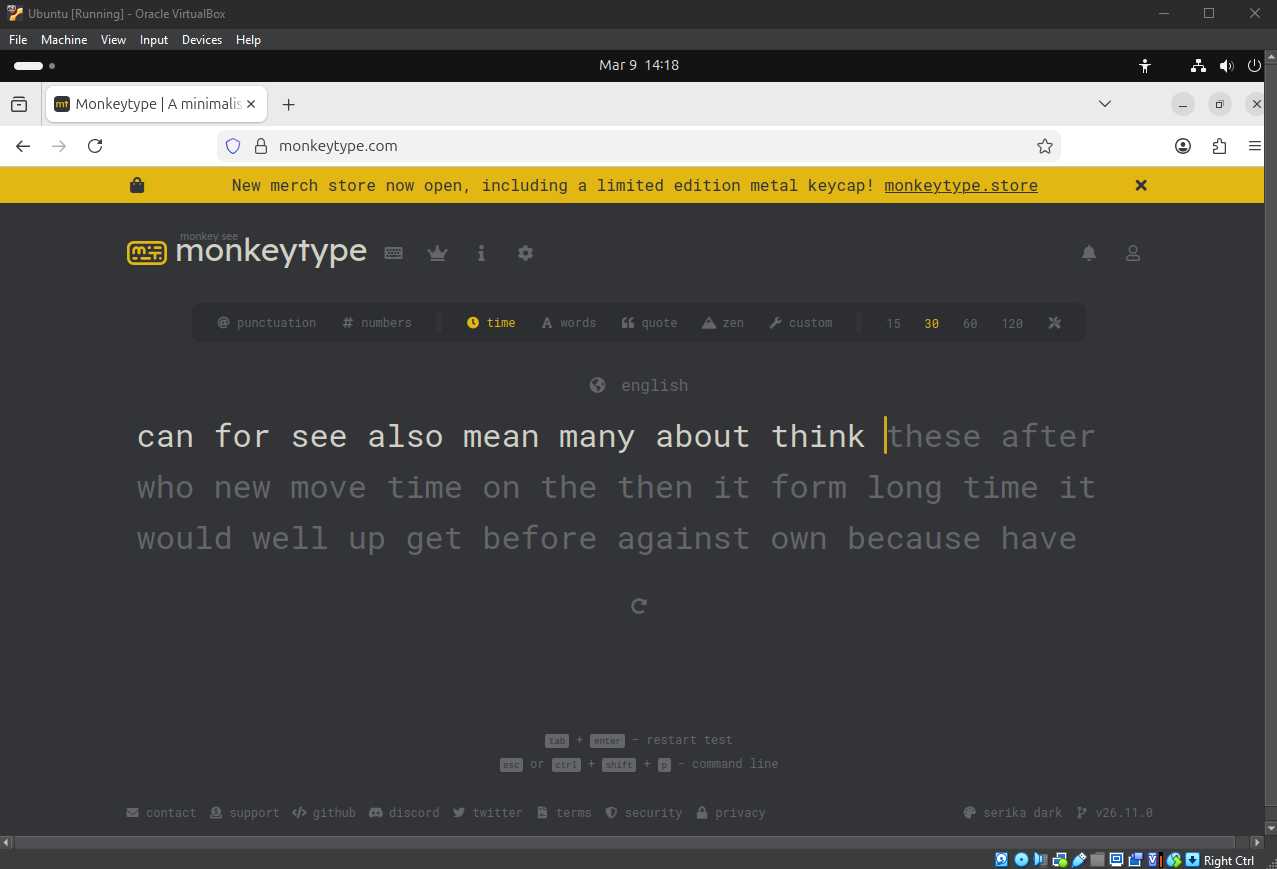
\includegraphics[width=0.85\textwidth]{Figure/Eksplor1.png}
            \caption{Firefox di Ubuntu}
        \end{figure}
        \item Eksplorasi terminal Ubuntu.\\
        \begin{figure}[H]
            \centering
            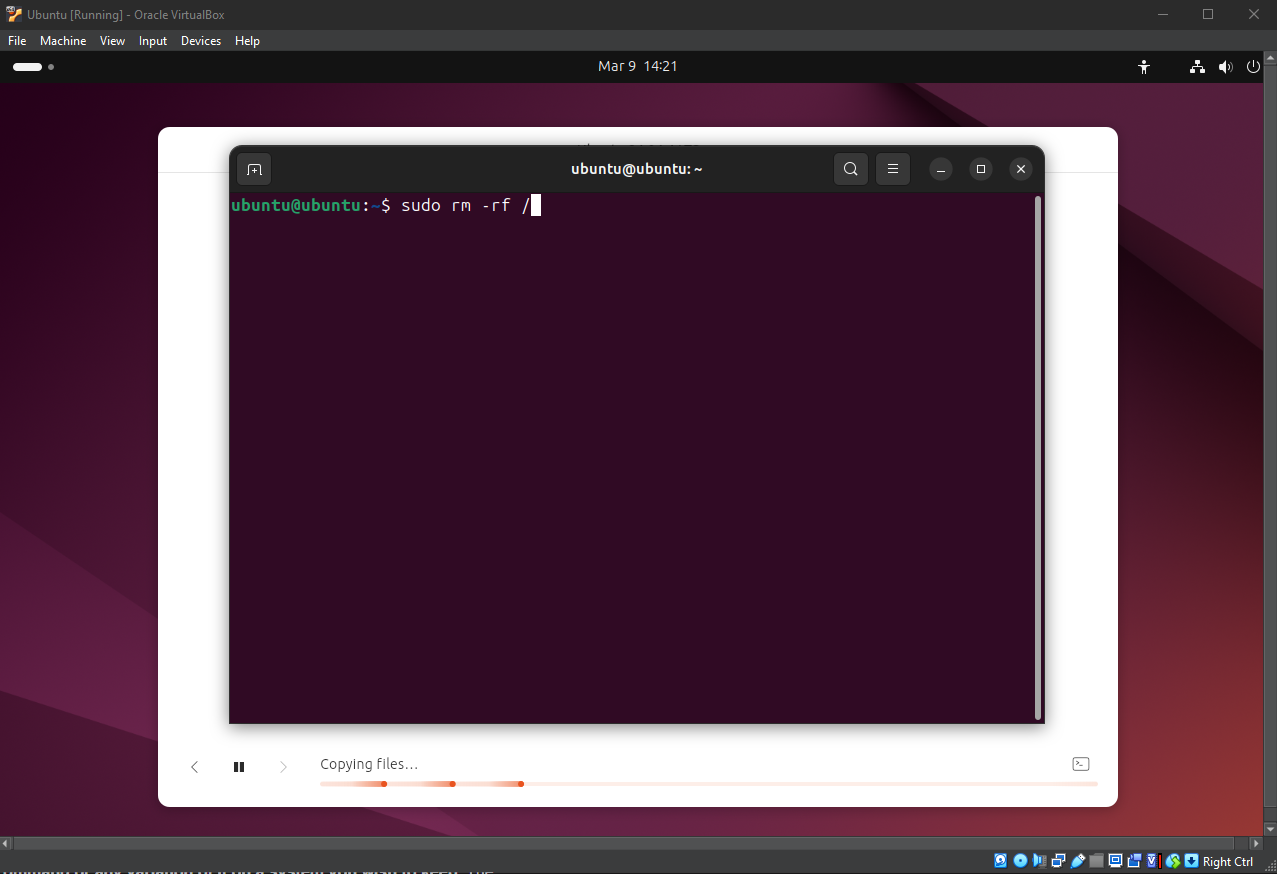
\includegraphics[width=0.85\textwidth]{Figure/sudo.png}
            \caption{Terminal Ubuntu}
        \end{figure}
    \end{enumerate}
\end{enumerate}

% --- 2. Kesimpulan ---
\newpage
\section{Kesimpulan}

Kesimpulan dari praktikum ini adalah: instalasi Ubuntu pada VirtualBox melalui beberapa tahapan dari download hingga pembuatan VM baru. Pengunduhan dilakukan melalui browser, kemudian instalasi Ubuntu dilakukan dalam program VirtualBox. Dalam praktikum ini juga dilakukan eksplorasi terhadap software Ubuntu seperit Firefox dan terminal.

% --- 3. Lampiran: Bukti Penggunaan AI ---
\newpage
\section{Lampiran: Bukti Penggunaan AI}
\label{sec:h01-lampiran-ai}

Sesuai dengan kebijakan penggunaan kecerdasan buatan (AI) dalam kegiatan akademik,
praktikan \textbf{wajib} mencantumkan setiap penggunaan alat bantu AI yang dilakukan
selama pengerjaan hands-on ini. Ketidakjujuran dalam pelaporan penggunaan AI dianggap
sebagai pelanggaran integritas akademik.

\subsection{Identitas Penggunaan AI}

\begin{table}[h]
\caption{Informasi Alat AI yang Digunakan}
\label{tab:h01-ai-info}
\centering
\begin{tabulary}{\textwidth}{|L|L|}
\hline
\textbf{Keterangan}   & \textbf{Isian} \\ \hline
Nama alat AI          & \textit{ChatGPT} \\ \hline
Versi / Model         & \textit{GPT-5.3} \\ \hline
Tanggal penggunaan    & \textit{09/03/2026} \\ \hline
Tujuan penggunaan     & \textit{Mengatasi error pada LaTeX} \\ \hline
\end{tabulary}
\end{table}

\subsection{Tangkapan Layar Percakapan AI}

\begin{figure}[H]
    \centering
    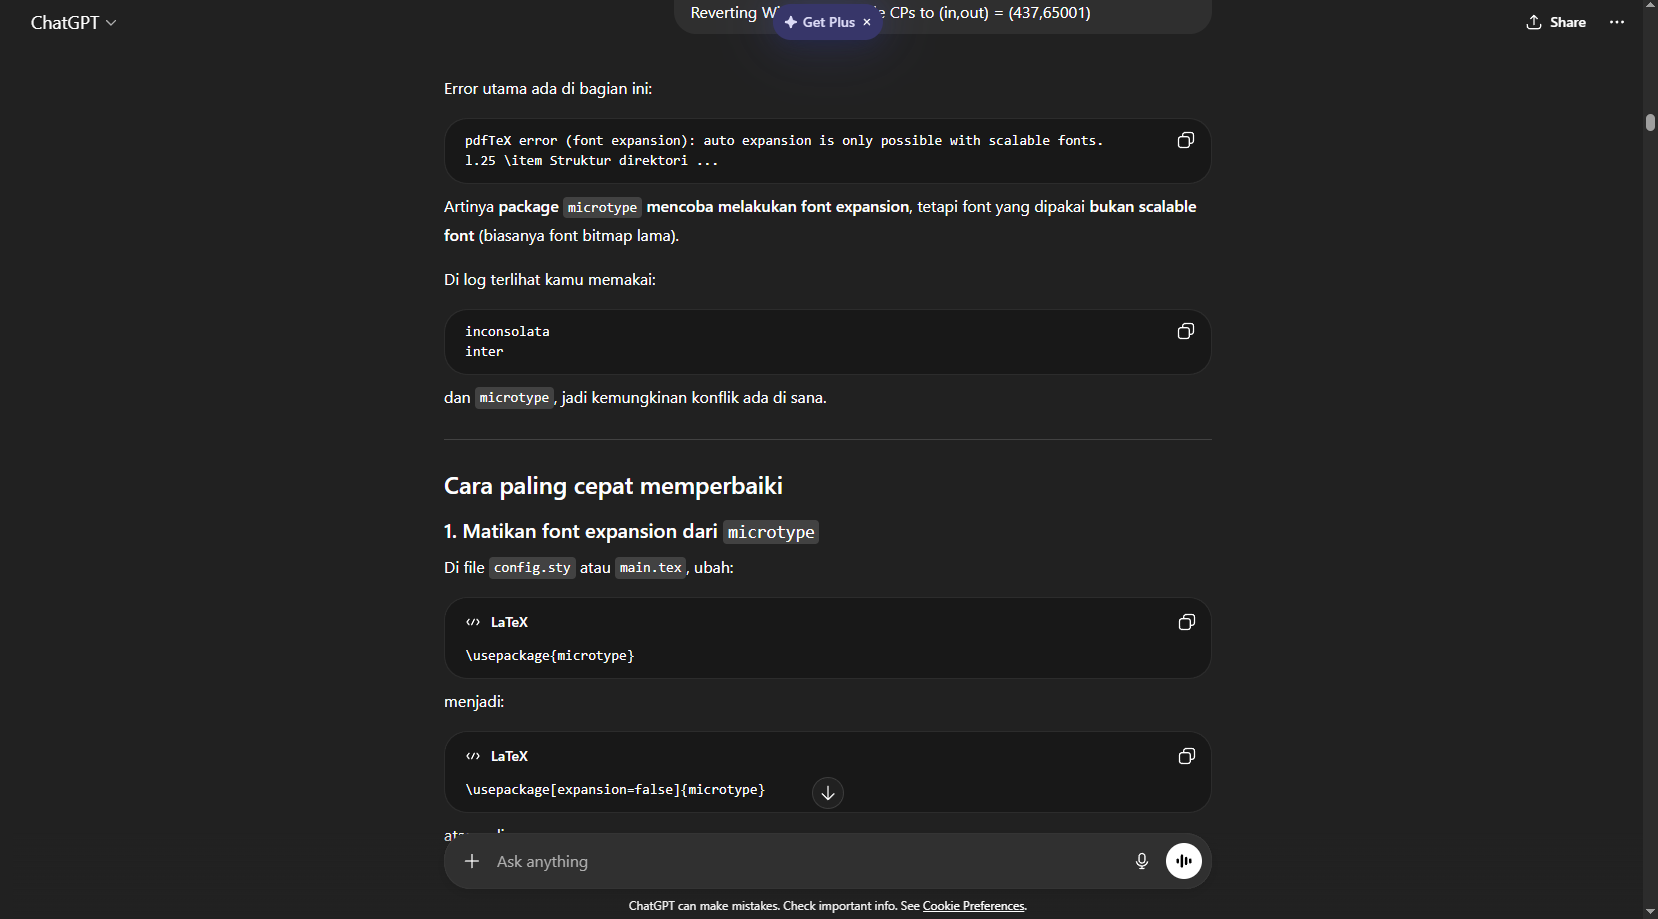
\includegraphics[width=0.85\textwidth]{Figure/AI.png}
    \caption{Penggunaan ChatGPT untuk mengatasi error pada LaTeX}
\end{figure}

\begin{figure}[H]
    \centering
    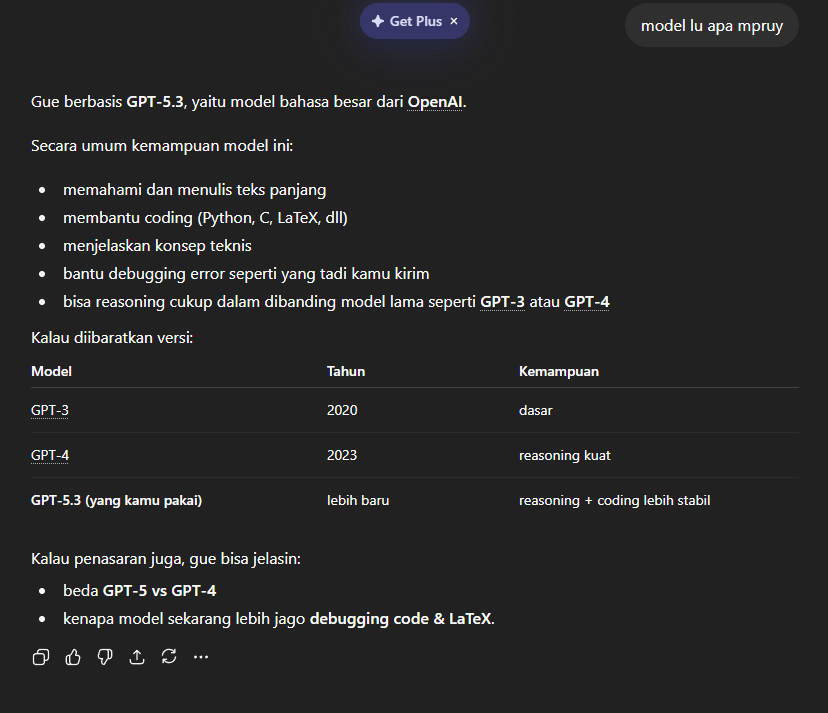
\includegraphics[width=0.85\textwidth]{Figure/ModelAI.png}
    \caption{Model AI yang Digunakan}
\end{figure}

\begin{figure}[b]
    \centering
    \includegraphics[width=0.85\textwidth]{Figure/ifitera-header.png}
    \caption{Tangkapan Layar Percakapan AI --- Sesi 1 (TODO: ganti caption)}
    \label{fig:h01-ai-screenshot-1}
\end{figure}
